\subsection{SDMetrics}
SDMetrics is a very complete design measurement tool, analysing a wide range of UML diagrams, including Class, Usecase, Activity and Statemachine diagrams.
For each type of diagram, this tool generates several metrics.\\
For example, \textbf{NumAttr} metric, one of the metrics that has already been adressed in this paper, is calculated from Class diagrams.
Other one is \textbf{ExtPts}, wich is calculated from Usecase diagrams, and gives us the number of extension points of a given use case.\\

SDMetrics is written in java, and provides us a graphical user interface. The type of source files it receives to analyse are \textit{XMI}\footnote{
\textit{XMI} (\textbf{X}ML \textbf{M}etadata \textbf{I}nterchange)  is an \textit{OMG} (Object Management Group) standard to generate
XML-based representations of UML and other OO data models.} files, most modeling tools support project exportation in XMI.\\
This tool allows us to access the results from different views. We will approach the ones that seem the most important:
\begin{itemize}
\item \textbf{Metric Data Tables} provides a table that matches each UML model element analysed (table line) to it's value for each metric (table column);
\item \textbf{Histograms} provides a graphical distribution  for each design metric;
\item \textbf{Design Comparison} provides us a mean to compare the structural properties of two \textit{UML} designs. It is very useful to compare the same design in different iterations of the development, or to compare an alternative design to the current one.
\item \textbf{Rule Checker} design rules and heuristics detect potencial problems in the UML design such as: 
	\begin{itemize}
	\item incomplete design such as unnamed classes, states without transitions;
	\item violation of naming conventions for classes, attributes, operations, packages;
	\item etc.
	\end{itemize}
\item \textbf{Catalog} this view provides us with the definitions of the metrics, design rules, and relation matrices for the current data set, and provides literature references and a glossary for them.
\end{itemize}
Not a view, but one of the most advanced features in this software is the possibility of defining Custom Design Metrics and Rules. The new metrics are defined in a XML file, with a very particular format, the \textit{SDMetricsML} (SDMetrics Markup Language). \\
The SDMetrics tool doesn't provide a direct notion of good/bad quality of the design model. Despite that, on the SDMetrics website we can find several indications of how to interpret each output. 
 
\subsubsection{Results}

Next we will show some printscreen's taken from SDMetrics, which will illustrate some of the outputs of this software, for our case-study.\\

\textbf{Metrics Table}
\begin{figure}[H]
\begin{center}
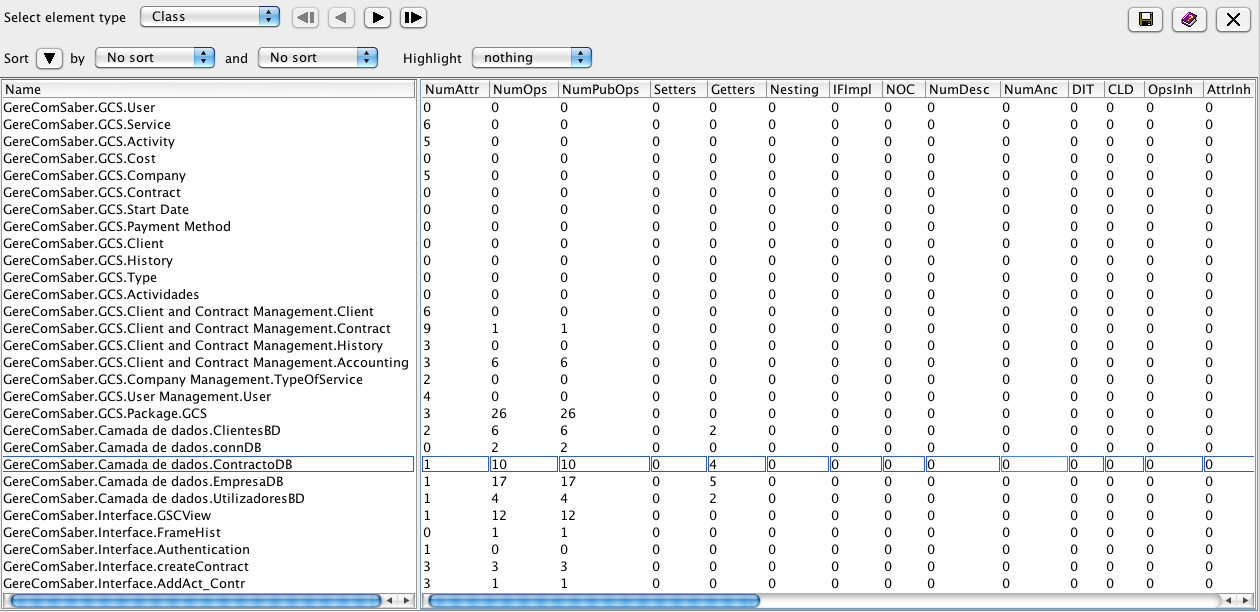
\includegraphics[width=1\textwidth]{images/table.png}
\caption{Metrics Table for class diagrams}\label{img:table}
\end{center}
\end{figure} 

\textbf{Histogram}
\begin{figure}[H]
\begin{center}
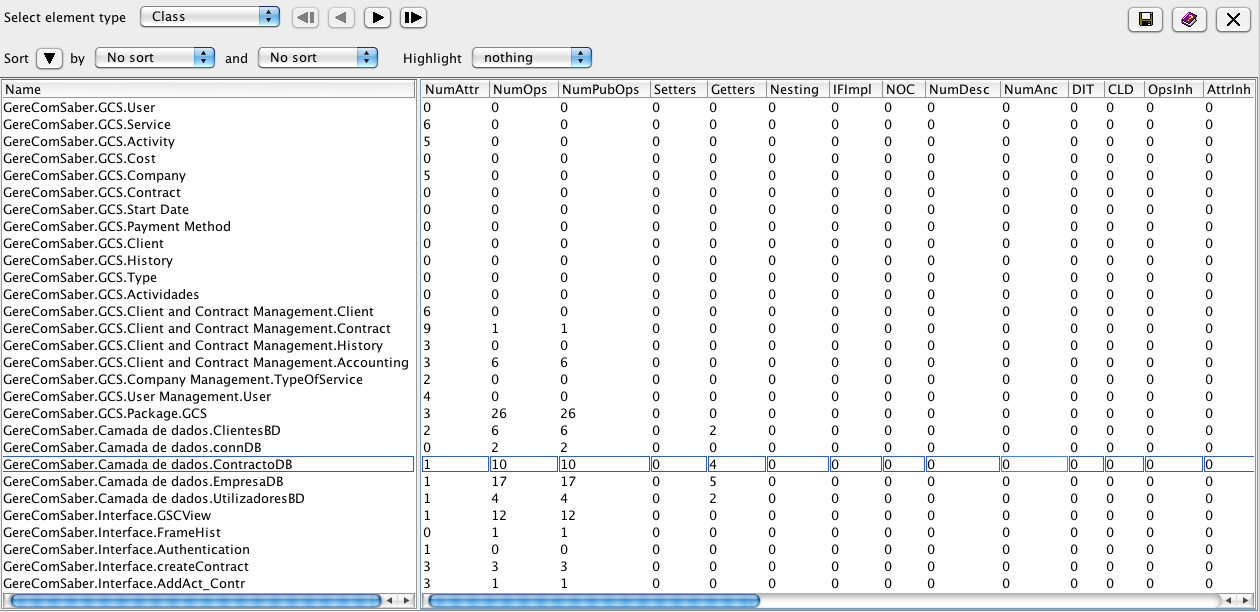
\includegraphics[width=1\textwidth]{images/table.png}
\caption{Histogram for class diagrams evaluating the metric NumAttr}\label{img:histogram}
\end{center}
\end{figure} 

\textbf{Rule Checker}
\begin{figure}[H]
\begin{center}
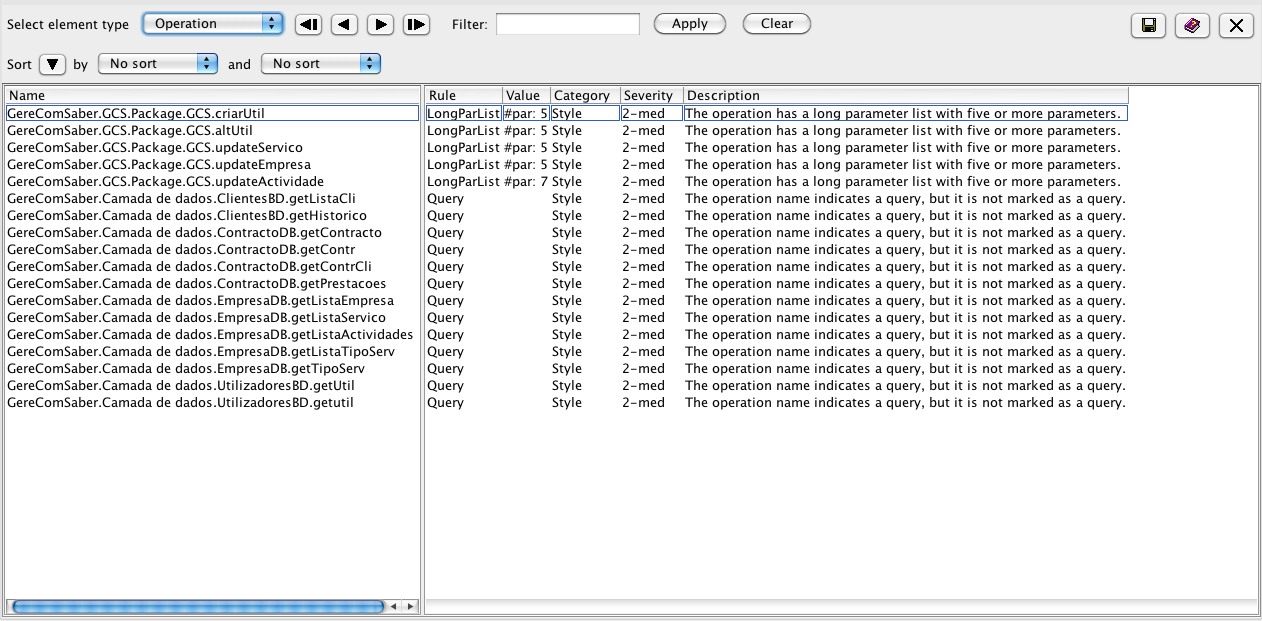
\includegraphics[width=1\textwidth]{images/rule.png}
\caption{Rule checking for Operations}\label{img:rule}
\end{center}
\end{figure} 